\subsection{Game Engine}
Game Enginen er skrevet i C\#, et objectorienteret programmering sprog
med stærkt library support der tillader udvikleren at fokusere på udvikling
af applikationer istedet for udvikling af libraries til at støtte projektet. \\

\noindent Nedstående præstenteres en diagram over de mest kritiske komponenter
Game Enginens interne spil logik og deres relationer til hinanden.
Der er ikke medtaget interfaces, eller klasser som er map, items, BackendController 
og logs som er mere specifikke til spillet og ikke til den interne logik.\\

\begin{figure}[h]
  \centering
   \caption{Viser det mest definerende elementer af Game Engine og deres relationerne til hinanden. Der er her ikke medtaget interface,
           abstract klasser, item, logs og map. }%
  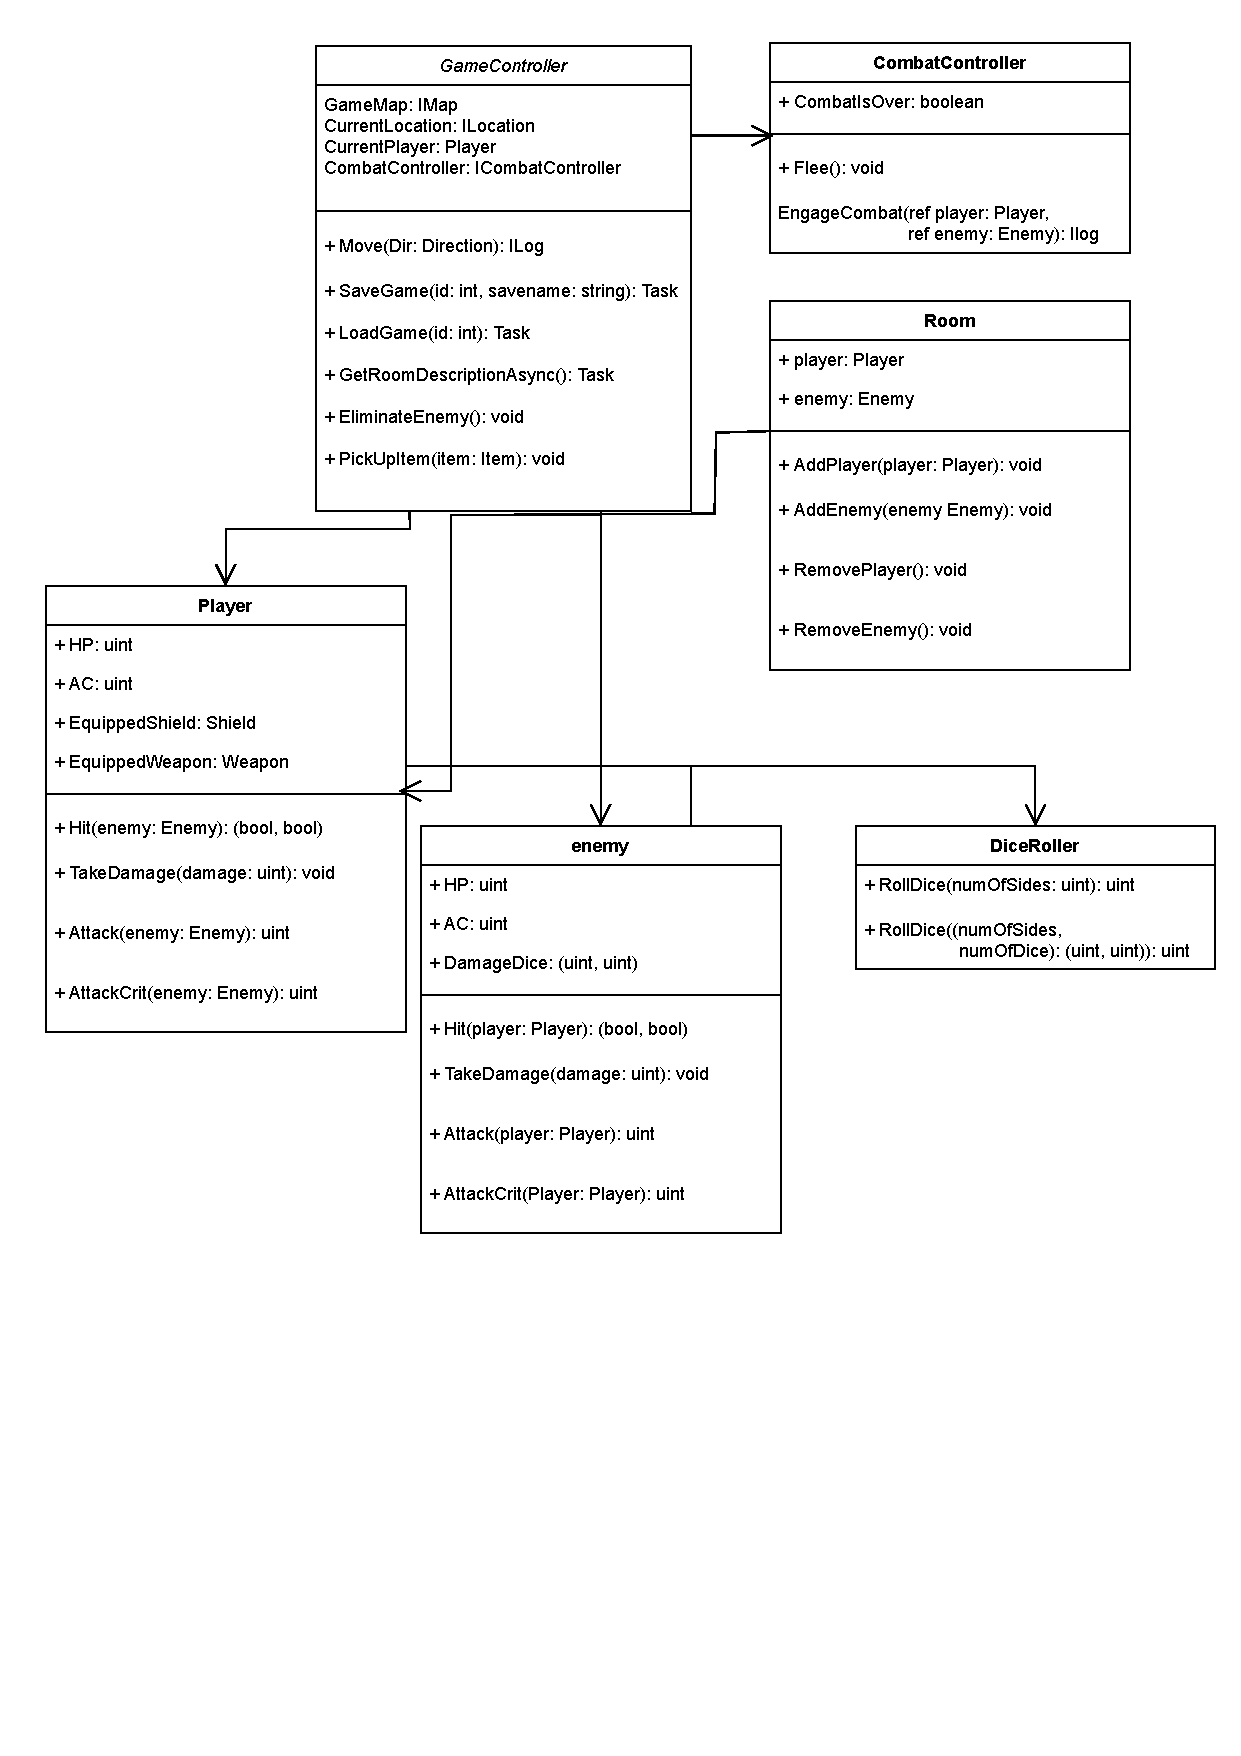
\includegraphics[width=0.9\linewidth, height=15cm, trim = 0 8cm 0 3cm]{02-Body/Implementering/GameEngineImplementering/Images/Core Class Diagram.pdf}
  \label{fig:CoreClassDiagram}
\end{figure}

\noindent GameControlleren er det centrale komponent i game enginen, denne er ansvarlig 
for kommunikation til frontend del af applikationen. I denne implementering af 
GameControlleren har den adgang til alle spillet funktionaliteter gennem dennes
association til Combatcontroller, se \autoref{fig:CoreClassDiagram}, og BackendController
, som ikke er vist på \autoref{fig:CoreClassDiagram}.

Fra et implementering perspektiv er dette en nem løsning for en lille applikationen som denne
men fra et design perspektiv er dette en dårlig løsning. GameControlleren har alt for mange
grunde til at ændre sig og følger næppe SOLID principperne.






